\documentclass[conference]{IEEEtran}

\ifCLASSINFOpdf
\else
\fi

\hyphenation{op-tical net-works semi-conduc-tor}

\usepackage{tikz}
\usetikzlibrary{arrows,positioning,automata}
\usepackage[noend]{algpseudocode}
\usepackage{algorithm}
\usepackage{enumitem, kantlipsum}

\begin{document}

\title{{\fontsize{19}{20}\selectfont Impact of Affective Appraisal
on Collaborative Goal Management:\\My Robot Shares My Worries}\vspace*{-5mm}}

 \author{\IEEEauthorblockN{Mahni Shayganfar and Charles Rich and
 Candace L. Sidner} 
 \IEEEauthorblockA{Computer Science Department,
 Worcester Polytechnic Institute\\
 100 Institute Road, Worcester, Massachusetts 01609-2280\\
 +1 (508) 831-5000\\
 \{mshayganfar , rich , sidner\}@wpi.edu}\vspace*{-10mm}}

%\author{Anonymous}

\maketitle

\begin{abstract}
A collaborative robot needs to be able to regulate and manage shared goals
during collaboration. Emotion has a crucial influence on this goal management
process. In this paper, we provide a cost function that we use to choose the
goal in the shared plan with the lowest cost value out of a set of alternative
goals. This cost function is a) based on the goal attributes, b) with respect to
the reverse appraisal of the perceived emotion, and c) the appraisal of the
collaborative environment.
\end{abstract}

\IEEEpeerreviewmaketitle
\vspace*{-2mm}
\section{Introduction}
\vspace*{-2mm}
Goals represent an important part of the context during collaboration. However,
not all goals are appropriate to pursue at the moment, depending on conditions.
In fact, it can be destructive for a collaboration to pursue a good goal in a
wrong context. Therefore, a collaborative robot must be able to manage shared
goals during collaboration. The goal management process provides a critical
influence on a collaborative robot's behavior by maintaining or shifting the
focus of attention to an appropriate goal based on the collaboration status.

Changes in a collaboration environment alter the balance of alternative goals.
These changes can reflect the collaborators' internal changes and the influence
of their actions. In a collaboration environment, emotions represent the outcome
of underlying mental processes of the collaborators. Emotions have many
different functions \cite{scheutz:architectural-action-selection} including
\textit{goal management}. Goal-oriented emotions such as anger, frustration and
worry regulate the mental processes influenced by one's internal goals. In our
example, a robot and an astronaut are collaborating to install solar panels.
When one of the astronaut's goals is blocked, the robot must manage the shared
goals in order to prevent failure of the collaboration. By using reverse
appraisal \cite{gratch:reverse-appraisal} of the astronaut's emotion and its
own appraisal of individual goals, the robot is able to successfully shift the
focus of attention from the blocked goal (eliciting worry in the astronaut) to
an appropriate one to maintain the collaboration.

\vspace*{-2mm}
\section{Contribution}
\vspace*{-1mm}
In this work, we focus on a small part of a larger framework based on our
\textit{Affective Motivational Collaboration Theory}
\cite{shayganfar:amct-symbiotic}. We introduce our goal management process based
on a cost function including the influence of affective appraisal and reverse
appraisal processes. Goal management is a crucial part of our investigation of
the reciprocal influence of appraisal on a collaboration structure (see Fig.
\ref{fig:actionSelection}).

\begin{figure}[tbh]
  \centering
  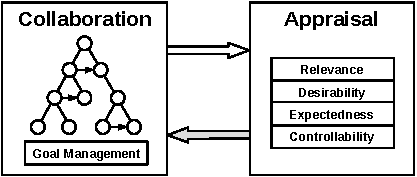
\includegraphics[width=0.37\textwidth]{figure/ActionSelection-croped.pdf}
  \vspace*{-2mm}
  \caption{{\fontsize{9}{9}\selectfont Reciprocal influence of Collaboration
  and Appraisal (mechanisms in our framework).}}
  \label{fig:actionSelection}
  \vspace*{-7mm}
\end{figure}

Appraisals are separable antecedents of emotion with which the robot
evaluates the environment. Our appraisal variables included: a)
\textit{relevance} to measure the significance of an event for the robot, b)
\textit{desirability} to characterize the value of an event to the robot in
terms of whether the event facilitates or thwarts the collaboration goal, c)
\textit{expectedness} and d) \textit{controllability} (these last two appraisal
variables are beyond the scope of this paper). The outcome of each appraisal
process is a specific value for the corresponding appraisal variable. The vector
containing these appraisal variables can be mapped to a particular emotion
instance at each point in time. However, it is not the actual emotion instance
that is important for us. In fact, it is a) the functions of emotions in a
social setting, i.e., goal management, and b) the meaning of the collaborator's
perceived emotion in collaboration context.

A collaboration structure provides a hierarchy and constraints of the shared
goals in the form of a shared plan (Fig. \ref{fig:taskModel}) which contains
both the robot and the human collaborator's goals. The robot pursues the goals
for which the robot is responsible in the shared plan. However, there can be
several live goals available for the robot to pursue at each point in time
during collaboration. A goal is \textit{live} if all of its
\textit{predecessors} are achieved and all of its \textit{preconditions} are
satisfied. Therefore, a collaborative robot requires a mechanism to choose
between a set of live goals. We believe appraisal processes are crucial to
choose between the available live goals, since the appraisals are the immediate
outcome of the robot's assessment of the collaboration environment.

For instance, Fig. \ref{fig:taskModel} shows a non-primitive ``Prepare Panels''
goal decomposed into three primitive goals. Therefore, if ``Prepare Panels'' is
live, its primitive goals can be pursued by the responsible agent. In our
example, the astronaut is responsible for the ``Check Connector'' goal; the
robot is responsible for the remaining two primitive goals. According to the
collaboration mechanism in our overall framework, ``Check Connector'' is in
focus, with the astronaut pursuing this goal. Suddenly, however the astronaut
tells the robot that she can not find the connector and she is \textit{worried}
about failure of this goal. The robot's response to this situation will be
explored below as we discuss details of our cost function.

\begin{figure}[tbh]
  \centering
  \vspace*{-1mm}
  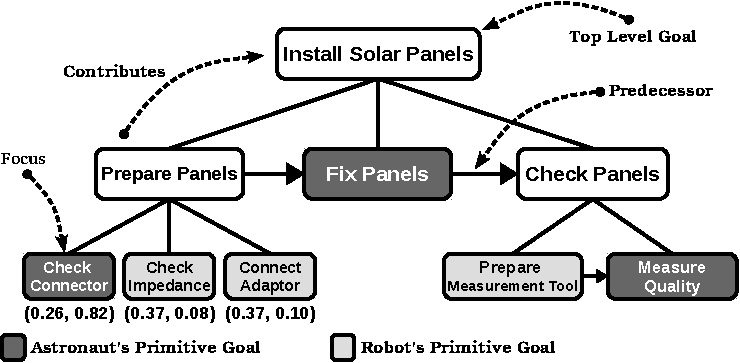
\includegraphics[width=0.48\textwidth]{figure/collaborationStructure-croped.pdf}
  \vspace*{-3mm}
  \caption{{\fontsize{9}{9}\selectfont Astronaut-robot collaboration structure
  (shared plan).}}
  \label{fig:taskModel}
  \vspace*{-3mm}
\end{figure}

Equation \ref{eqn:cost} shows the function to calculate the cost of each
live goal. The base in the equation calculates the cost of pursuing any given
goal. The three functions used to calculate the cost are:
\textit{proximity} $P(g)$, \textit{difficulty} $D(g)$, and \textit{specificity}
$S(g)$ (see equations \ref{eqn:proximity} to \ref{eqn:specificity}).

\vspace*{-6mm}
\begin{equation}
{\fontsize{6}{9}\selectfont Cost(g) =
\big(\omega_0.P(g)+\omega_1.D(g)+\omega_2.\frac{1}{S(g)+1}\big)}^{\Gamma}
\label{eqn:cost}
\vspace*{-1mm}
\end{equation}

\noindent For simplicity, we assume equal values for the weights: $\omega_i$=1.

\vspace*{-2mm}
\begin{equation}
\Gamma=-C[(R_r+1)D_r + \alpha(R_h+1)D_h]
\label{eqn:power}
\vspace*{-2mm}
\end{equation}

The exponent part of our cost function (Equation \ref{eqn:power}) captures a)
the influence of the human's perceived emotional instance, and b) the influence
of self appraisal of the given goal. $R_h\in[0,1]$ and $D_h\in[-1,1]$ are the
relevance and desirability values respectively, which are based on the
\textit{reverse} appraisal of the human's perceived emotion. For instance, if
the astronaut is \textit{worried}, $D_h$ is negative, e.g., -0.8 (depending on
how undesirable the event is according to reverse appraisal), and $R_h$ will be
1 for the active goal and its value descends to 0 for other live goals depending
on their distance to the active goal in the shared plan (e.g., 0.1).

$R_r\in[0,1]$ and $D_r\in[-1,1]$ are relevance and desirability values, provided
by the \textit{self} appraisal functions for all of the live goals. For
instance, for the active goal for which the astronaut was \textit{worried},
$D_r$ can be positive, e.g., 0.8 (depending on the self's desirability appraisal
function); $R_r$ can be 1, since the active goal is relevant for the robot.
These values will change for the other live goals depending on how
relevant they are with respect to the collaboration status (e.g., 0.9 and 0.8).
Finally, $C\in[1,\infty)$ is a constant (e.g., 2) used to control the influence
of affect on cost value. It is negative since undesirability (negative values)
should increase the cost. $\alpha\in[1,\infty)$ is another constant (e.g., 3)
used to control the importance of reverse appraisal relative to self appraisal.

The \textit{proximity} of a goal indicates how far the goal is from the current
active goal in the shared plan. It is calculated by the distance function
(Equation \ref{eqn:proximity}) which returns the number of edges between the
current active goal $g_{_{act}}$, and the given goal $g$ in the shared plan. In
our example, $P(g)$ is 2 for both ``Check Impedance'' and ``Connect Adaptor''
goals.

\vspace*{-3mm}
\begin{equation}
P(g) = max\big\{1, distance(g_{_{act}},g)\big\}
\label{eqn:proximity}
\vspace*{-1mm}
\end{equation}

The \textit{difficulty} of a goal is a function of three parameters (Equation
\ref{eqn:difficulty}) which consider the difficulty based on a) topology of the
shared plan tree (domain independent), and b) the amount of effort required to
pursue a given goal (domain dependent). The $\sum pred_e(g)$ is the sum of
efforts that all the \textit{predecessors} of a given goal $g$ require. The
$\sum desc_e(g)$ is the sum of efforts that all the \textit{descendants} of a
given goal $g$ require. The effort values represent the amount of effort for the
goals with respect to the domain. In our example, we assume the values of all
the goal efforts are 1 for simplicity. The $H(g)$ is the height of the given
goal $g$. The heights of all primitives under ``Prepare Panel'' goal are 0 in
our example.

\vspace*{-5mm}
\begin{equation}
D(g) = \Big(H(g)+1\Big)\times\left[\sum\limits_{m=0}^{M} pred_e(g) +
\sum\limits_{n=0}^{N} desc_e(g)\right]
\label{eqn:difficulty}
\end{equation}

The \textit{specificity} of a goal is the function of \textit{depth} (distance
from the root) and \textit{degree} (number of children) of a given goal $g$. The
first non-primitive goal (root) is the least specific goal, and the
primitives (leaves) are the most specific goals. As calculated based on Fig.
\ref{fig:taskModel}, the values of $S(g)$ for the three primitives under the
``Prepare Panels'' are 2.

\vspace*{-2mm}
\begin{equation}
S(g) = \frac{depth(g)}{degree(g)+1}
\label{eqn:specificity}
\end{equation}

\vspace*{-1mm}
The tuples below the goals in Fig. \ref{fig:taskModel} indicate the cost value
of each goal. The first number in each tuple is the normalized cost value
without the influence of the affective part of the cost function, i.e., the
exponent is equal to 1 in Equation \ref{eqn:cost}. The second number of each
tuple indicates the normalized value of the cost including the influence of
affective appraisal and the astronaut's perceived emotion.

Based on our cost function, the cost of completing the primitive goal ``Check
Connector'' is 0.82 (see Fig. \ref{fig:taskModel}). As shown, when affect is
not considered the cost is 0.26; the negative emotion of the astronaut (worry)
significantly increases the cost of the current goal, and also impacts the other
two primitive live goals under the same parent. Therefore, instead of insisting
on pursuing the same blocked goal which has caused the astronaut's negative
emotion, the robot can mitigate the astronaut's emotions by adapting to her
worry. The robot shifts the focus of attention to ``Check Impedance'' to
maintain progress and prevent failure of the collaboration. The details about
the robot's behavior is beyond the scope of this paper.

\vspace*{-1mm}
\section{Conclusion}
\vspace*{-1mm}
We use our proposed cost function in our goal management algorithm to be able to
integrate affective appraisal into the collaboration mechanism in our framework.
We will evaluate our cost function through conducting a user study to compare
our results with humans' responses. We will continue to implement other parts of
our framework, including action selection and motivation processes.
\vspace*{-1mm}

\bibliographystyle{IEEEtran}
\bibliography{mshayganfar.bib}

\end{document}